\documentclass{beamer}
\mode<presentation>
\usetheme{CambridgeUS}
\usecolortheme{beaver}

\usepackage[english]{babel}
\usepackage{graphicx}
\usepackage{subfigure}
\usepackage[backend=bibtex]{biblatex}
\bibliography{bibliography}

\title[Dynamic Routing Between Capsules]{Dynamic Routing Between Capsules}
\author[Mu\c sat Bogdan-Adrian]{Authors: Sara Sabour, Nicholas Frosst, Geoffrey E Hinton}
\date{November 2017}

\beamertemplatenavigationsymbolsempty
\graphicspath{{./images/}}

\begin{document}

\frame{\titlepage}

\begin{frame}
\frametitle{Introduction}
\center
\begin{itemize}
	\item A capsule is a group of neurons whose activity vector represents an entity - 				  either an object or an object part
	\item The length of the vector represents the probability that a certain entity exists
	\item Achieves state-of-the-art performance on MNIST and is better at recognizing highly 			  overlapping digits than a convolutional network
\end{itemize}
\end{frame}

\begin{frame}
\frametitle{Reference With Human Vision}
\center
\begin{itemize}
	\item The human vision processes only a tiny fraction of the optic array at the highest 			  resolution
	\item Assumption that the visual system creates a parse tree on each fixation
	\begin{figure}
	\subcapcentertrue
    \centering
    	\subfigure[Parse tree example: \newline (7 + 3) * (5 - 2)]
        {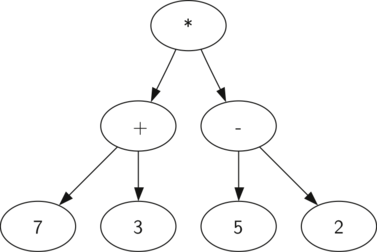
\includegraphics[width=0.4\textwidth]{parse_tree.png}}
    \end{figure}
\end{itemize}
\end{frame}

\begin{frame}
\frametitle{Capsules as Parse Trees}
\center
\begin{itemize}
	\item A parse tree can be represented by a multilayer neural network
	\item Each layer will be divided into many capsules
	\item Using an iterative routing process, each capsule will choose a capsule in the layer above to be its parent in the tree - this process solves the problem of assigning parts to wholes
\end{itemize}
\end{frame}

\begin{frame}
\frametitle{Describing the Capsule}
\center
\begin{itemize}
	\item The vector of activities of a capsule represent the various properties of a particular entity that is present in the image (pose, deformation, velocity, texture etc.)
	\item The existence of an object is defined by using the overall length of the activity vector of a capsule - a non-linearity is applied so that the length of the vector output cannot exceed 1
	\item A lower level capsule is assigned to a higher level capsule by a "routing-by-agreement" algorithm
\end{itemize}
\end{frame}

\end{document}
